\documentclass[a4paper, 12pt]{report}
\usepackage[utf8]{inputenc}
\usepackage[T2A]{fontenc}
\usepackage[english,russian]{babel}
\usepackage[dvips]{graphicx}
\usepackage[left = 2cm, top = 1cm, right = 2cm, bottom = 2cm]{geometry}
\usepackage{hyperref}
% \usepackage{xcolor}
\usepackage{titlesec}
\usepackage{listings}
\usepackage{amsmath}
\usepackage{eufrak}
\usepackage{amsthm}
\usepackage{dsfont}

\usepackage{color}

\usepackage{shortcuts}

\newtheorem{definition}{Определение}[chapter]
\newtheorem*{theorem}{Теорема}
\newtheorem{St}{Утверждение}[chapter]

\lstloadlanguages{C,[ANSI]C++}%,Clean,make,Fortran}%Загружаемые языки
\lstset{extendedchars=false,
        breaklines=true, %автоперенос длинных линий
        breakatwhitespace=true}
\graphicspath{{pic/}}
\titleformat{\chapter}[block]{\color{black}\Large\bfseries\filcenter}{}{1em}{}
\setcounter{secnumdepth}{0}


\begin{document}
\title{Основания алгебраического подхода к синтезу корректных алгоритмов}
\author{Лектор --- Рудаков К.В.\\ Наборщик --- Старожилец В.М.}
\date{}
\maketitle

\tableofcontents

\chapter{Лекция 1}
\section{Введение}
Данные лекции рассматривают общую задачу машинного обучения без привязки к конкретным методам и основы алгебраического подхода к синтезу корректных алгоритмов для её решения. В некотором роде они являются взглядом сверху на задачи машинного обучения и методы их решения.

В первую очередь следует сформулировать задачу машинного обучения в общем виде. По сути это задача построения алгоритма, который реализует отображение из множества начальных информаций в множество конечных информаций. Сразу отметим, что в курсе рассматриваются только такие отображения, для которых существует реализующий их алгоритм.

\begin{definition}
Символом $\mathfrak{I_i}$ (читается <<И инишл>>) будем обозначать множество начальных информаций, например, симптомы болезни.
\end{definition}

\begin{definition}
Символом $\mathfrak{I_f}$ (читается <<И файнэл>>) будем обозначать множество конечных информаций, например, диагноз.
\end{definition}

Таким образом, на формальном языке нам требуется найти такой алгоритм $A$, что он осуществляет отображение из множества начальных информаций $\mathfrak{I_i}$ в множество конечных информаций $\mathfrak{I_f}$:
\[
A: \mathfrak{I_i} \rightarrow \mathfrak{I_f}.
\]
Пока что задача стоит так, что нам нужно найти некоторое произвольное отображение из одного множества в другое, реализуемое некоторым алгоритмом. При этом свойства этого отображения и алгоритма неважны. В такой постановке у нас нет каких-либо ограничений на искомый алгоритм: даже датчик случайных чисел является решением этой задачу. Поэтому вводятся дополнительные ограничения на допустимые алгоритмы. Итак,

\begin{definition}
Обозначим $\mathfrak{M}^* = \{A|\ A:\  \mathfrak{I_i}\rightarrow \mathfrak{I_f}\}$ множество всех алгоритмов, реализующих отображение из $\mathfrak{I_i}$ в $\mathfrak{I_f}$.
\end{definition}

\begin{definition}
Обозначим $I_{str}$ структурную информацию, содержащую условия и требования, накладываемые на $A$.
\end{definition}

\begin{definition}
Обозначим $\mathfrak{M}(I_{str}) \subset \mathfrak{M}^*$ некоторое подмножество $\mathfrak{M}^*$, удовлетворяющее $I_{str}$.
\end{definition}

Теперь у нас есть дополнительная информация $I_{str}$, позволяющий накладывать дополнительные ограничения на нашу задачу. Введём определения допустимого отображения и корректного алгоритма.

\begin{definition}
Любое отображение из множества $\mathfrak{M}(I_{str})$ называется допустимым.
\end{definition}

\begin{definition}
Задача Z заключается в построении алгоритма, реализующего допустимое отображение.
\end{definition}

\begin{definition}
Любой алгоритм реализующий любое допустимое отображение называется корректным.
\end{definition}

В такой формулировке необходимым и достаточным условием разрешимости задачи Z является выполнение выражения: \[
\mathfrak{M}(I_{str}) \neq \emptyset,
\]
а условием единственности решения~--- выполнение равенства:
\[
|\mathfrak{M}(I_{str})| = 1.
\]
Заметим также, что в данной формулировке корректный алгоритм~--- это алгоритм, не допускающий ни одной ошибки, а множество $\mathfrak{M}(I_{str})$~--- множество алгоритмов не допускающих ошибок. Однако можно поставить условия несколько мягче, и дать алгоритмам возможность ошибаться.

\section{Поиск решения задачи}
Пусть $\mathfrak{M}(\pi)$~--- некоторое параметрическое семейство отображений. После того как мы выбрали некоторое семейство отображений $\mathfrak{M}(\pi)$, попытаемся попасть в $\mathfrak{M}(I_{str})$, взяв в $\mathfrak{M}(\pi)$ какое-нибудь отображение за начальное. Это возможно, если данные семейства пересекаются:
\[
\mathfrak{M}(\pi) \cap \mathfrak{M}(I_{str}) \neq \emptyset.
\]

Но, с одной стороны, чем \emph{сложнее} наше семейство, тем выше вероятность, что оно пересекается с семейством $\mathfrak{M}(I_{str})$, однако, с другой стороны, достижение этого пересечения может быть \emph{затратно}, если $\mathfrak{M}(\pi)$ сложное. Также всегда остаётся вероятность, что множество $\mathfrak{M}(\pi)$ с $\mathfrak{M}(I_{str})$ не пересекается. Для поиска компромиссного решения используют идею \emph{расширения множества}.

\begin{definition}
Пусть $f$~--- некоторая операция над множеством $\mathfrak{M}^*$. Тогда $f(\mathfrak{M}(\pi))$ будем называть расширением множества $\mathfrak{M}(\pi)$.
\end{definition}

Таким образом, мы хотим расширить некоторое <<простое>> множество до пересечения с $\mathfrak{M}(I_{str})$. Однако, не любая функция $f$ нам подходит, так как <<простое>> множество может расшириться до слишком <<сложного>> множества. Важно, что $f$ мы выбираем сами, поэтому можем выбрать его так, чтобы искать нужный алгоритм было не слишком сложно.

\chapter{Лекция 2}
\section{Алгебра, реляционная система и алгебраическая система}
Данная лекция посвящена вопросам терминологии, используемой в данном курсе. Поэтому тут будет очень много определений (ещё больше, чем в предыдущей). Для начала определим понятия алгебры, реляционной системы и алгебраической системы.

\begin{definition}
Сигнатура~---набор характеристик, однозначно идентифицирующий объект.
\end{definition}

\begin{definition}
Отношение~--- математическая структура, которая формально определяет свойства различных объектов и их взаимосвязи. В нашем курсе будет обозначаться буквой $R$.
\end{definition}

\begin{definition}
Алгеброй называется структура
\[
\left(
\begin{array}{ccccc}
  A & Op_1 & Op_2 & ... & Op_k \\
    & n_1 & n_2 & ... & n_k
\end{array}
\right)
\]
где A~--- множество, $Op_i$~--- операции на этом множестве, $n_i$~--- сигнатуры.
\end{definition}

\begin{definition}
Реляционной системой называется структура
\[
\left(
\begin{array}{ccccc}
  A & R_1 & R_2 & ... & R_k \\
    & n_1 & n_2 & ... & n_k
\end{array}
\right)
\]
где A~--- множество, $R_i$~--- отношения на этом множестве, $n_i$~--- сигнатуры.
\end{definition}

\begin{definition}
Алгебраической системой называется структура
\[
\left(
\begin{array}{ccccccccc}
  A & R_1 & R_2 & ... & R_k & Op_1 & Op_2 & ... & Op_l \\
    & n_{1,1} & n_{1,2} & ... & n_{1,k} & n_{2,1} & n_{2,2} & ... & n_{2,l}
\end{array}
\right),
\]
где A~--- множество, $R_i$~--- отношения на этом множестве, $Op_i$~--- операции на этом множестве, $n_i$~--- сигнатуры.
\end{definition}

\section{Первичные свойства функции}
Теперь поговорим о функциях. Первичные свойства функций~--- это иньективность, сурьективность и биективность. Все остальные свойства требуют задать некоторую структуру на тех множествах, на которых они действуют (например, метрику).
Пусть функция~$f$ действует из~$A$ в $B$. То есть:
\[
\left\{
  \begin{array}{ll}
    f: A\rightarrow B\\
    f(A) \subseteq B
  \end{array}
\right.
\]
Определим также понятие отношения эквивалентности на множестве $A$:

\begin{definition}
Отношением эквивалентности $\pi_f$ на множестве $A$ называется бинарное отношение, которое обладает свойствами транзитивности, симметричности и рефлексивности.
\end{definition}

Данное определение приводит нас к определению фактор-множества $A_{\pi_f}$ и ядерной эквивалентности отображения $f$.

\begin{definition}
Фактор-множество $A_{\pi_f}$~--- это множество всех классов эквивалентности заданного множества $A$, по заданному отношению $\pi_f$.
\end{definition}

\begin{definition}
Ядерная эквивалентность отображения $f$:
\[
(a_1\equiv a_2)\equiv(f(a_1)=f(a_2)),
\]
где эквивалентность понимается в смысле $\pi_f$. Следует понимать, что мы выбираем $\pi_f$ так, чтобы это свойство было выполнено. Это выполнено не для любого отношения эквивалентности.

\textcolor{red}{Саня, тут надо как нибудь переписать... непонятно что откуда идет. Я так понимаю что мы $\pi_f$ выбираем по f, но чёрт его знает.}
\end{definition}

Таким образом, мы можем, например, показать, что любое отображение из $A$ в $B$ раскладывается в суперпозицию суръекции, инъекции и биекции. Данный факт легко понять с помощью рисунка~\ref{fig::superpos}:

\begin{figure}[htbp]
\centering
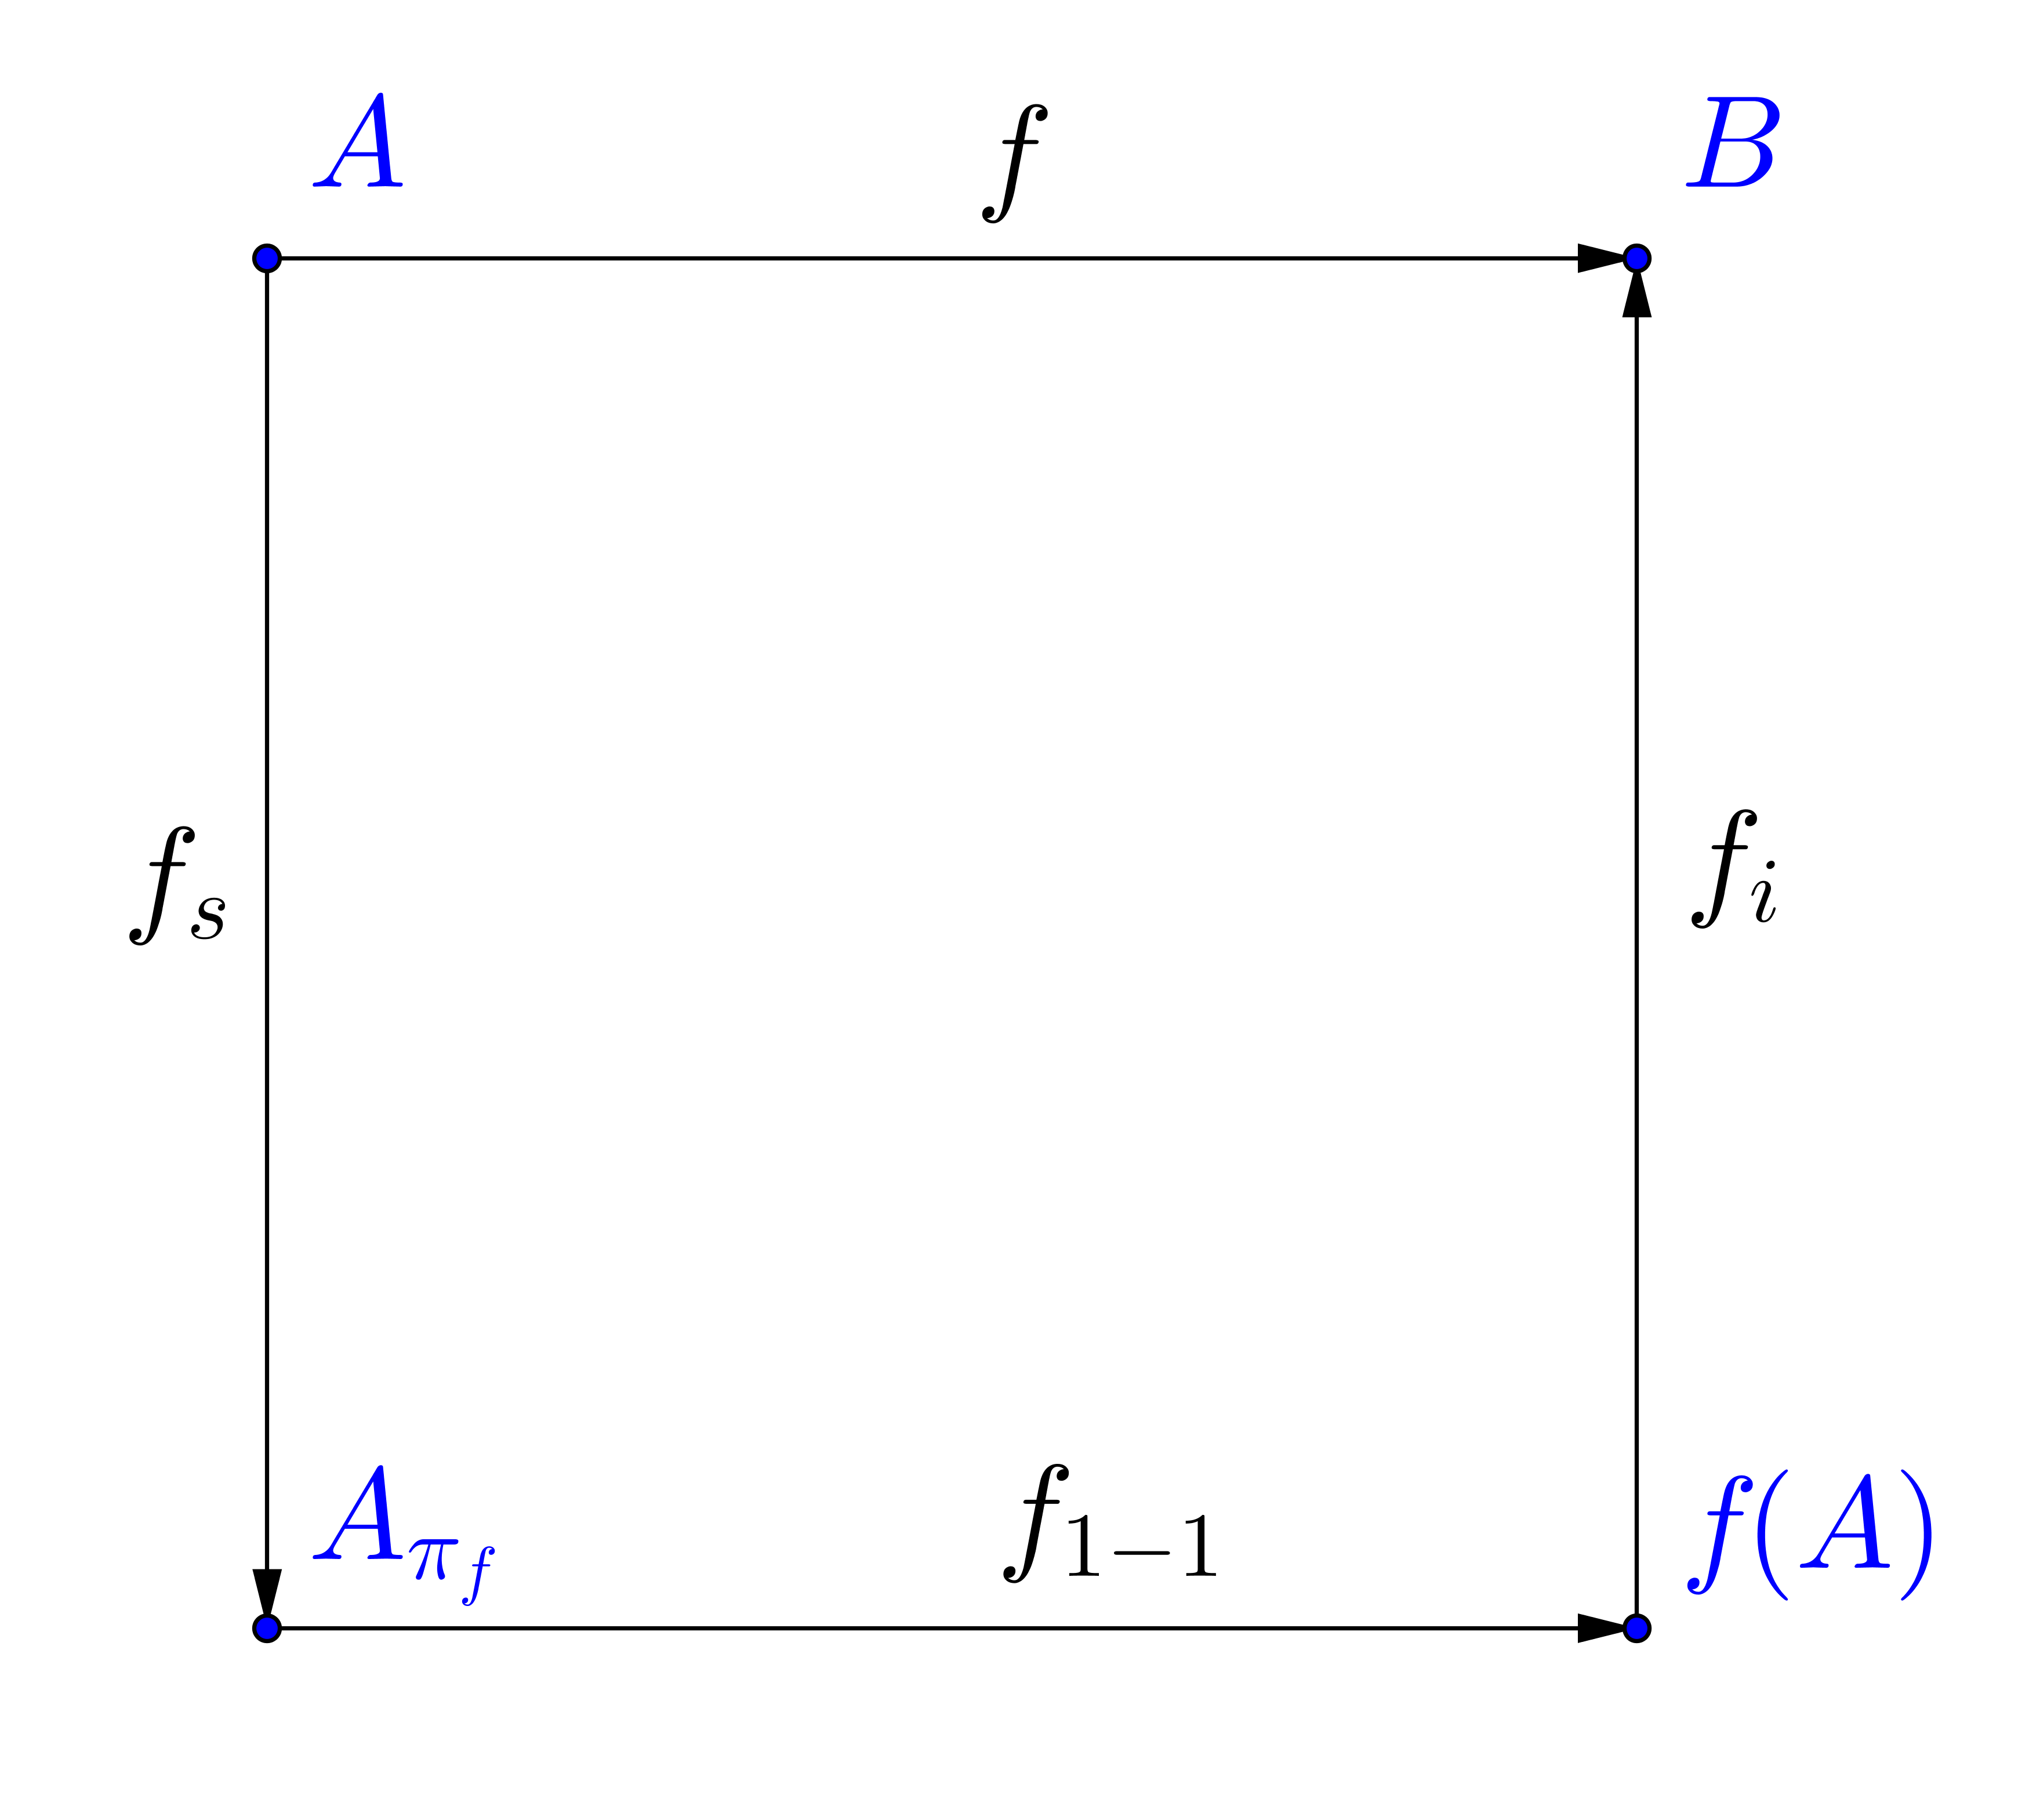
\includegraphics[width=0.6\linewidth]{lect2/InectBiectSuriect.png}
\caption{Иллюстрация представления отображения $f$ как суперпозиции суръекции, инъекции и биекции. $f_S$~--- суръекция, $f_{1-1}$~--- биекция, $f_i$~--- инъекция}
\label{fig::superpos}
\end{figure}

На рис.~\ref{fig::superpos} изображены четыре множества: $A$, $B$, $A_{\pi_f}$~---фактор-множество, и $f(A)$. Множество $A$ суръективно отображается в свое фактор-множество $A_{\pi_f}$, из-за ядерной эквивалентности отображения $f$, $A_{\pi_f}$ биективно отображается в $f(A)$. В свою очередь $f(A)$ иньективно вкладывается в $B$ как его подмножество.

\section{О декартовом произведении множеств}
Поговорим о декартовом произведении множеств и о том, как его можно представить через другие операции с множествами. Итак, пусть есть множество индексов $\mathfrak{A} = \{\alpha\}$ и соответствующий этому множеству индексов набор множеств $\{A_{\alpha}|\ \alpha \in \mathfrak{A}\}$. Чему тогда равно произведение $\prod_{\alpha \in \mathfrak{A}}A_{\alpha}$? По крайней мере оно ненулевое, так как любое декартово произведение произвольного семейства непустых множеств в непустом количестве непусто (об этом свидетельствует аксоима выбора). Оказывается, что
\[
\prod_{\alpha \in \mathfrak{A}}A_{\alpha} = \{f|\ f:\ \mathfrak{A}\rightarrow\bigcup_{\alpha \in \mathfrak{A}}A_{\alpha}, \forall\alpha\in\mathfrak{A}: f(\alpha)\in A_{\alpha}\}
\]

Например, пусть
\[
A_{\alpha} = A_{(x, y)} = \{(x', y')| \rho((x,y), (x',y')) \leq 1\}
\]
Тогда
\[
\prod_{\alpha \in \mathfrak{A}}A_{\alpha} = \{f| f: R^2 \rightarrow R^2,\ \forall (x,y): \rho((x,y), f((x,y))) \leq 1\}
\]

\chapter{Лекция 3}
\section{Свободное произведение}
\textcolor{red}{Саня, Я вообще не уверен, что тут все правильно. Проверь меня, если сам понял хоть что-то в этой теме:). Надо ещё как то обосновать представление прямой суммы как специфического объединения. Я не понял почему оно так представляется. Очень может быть что я пропустил тут в определениях какое нибудь "для любого альфа", мне самому не совсем понятно}

Прежде чем вводить свободное произведение, вспомним о понятии гомоморфизма, играющем важную роль в свободном произведении.

\begin{definition}
Гомоморфизм~--- это отображение алгебраической системы $A$, сохраняющее основные операции и основные соотношения\footnote{Уточнить!}.
\end{definition}

\begin{definition}[Свободное произведение]
Пусть имеется $\{A_{\alpha}|\ \alpha\in\mathfrak{A}\}$~--- некоторое множество алгебраических систем. Тогда алгебраическая система $B$, порождённая системами $A_{\alpha}$ так, что гомоморфизм $\varphi_{\alpha}: C \rightarrow A_{\alpha}$, где $C$~--- произвольная алгебраическая система, продолжается до гомоморфизма $f:\ C\rightarrow B$ называется свободным произведением и обозначается
\[
\prod_{\alpha\in\mathfrak{A}}^* A_{\alpha}.
\]
\end{definition}

\begin{figure}[htbp]
\centering
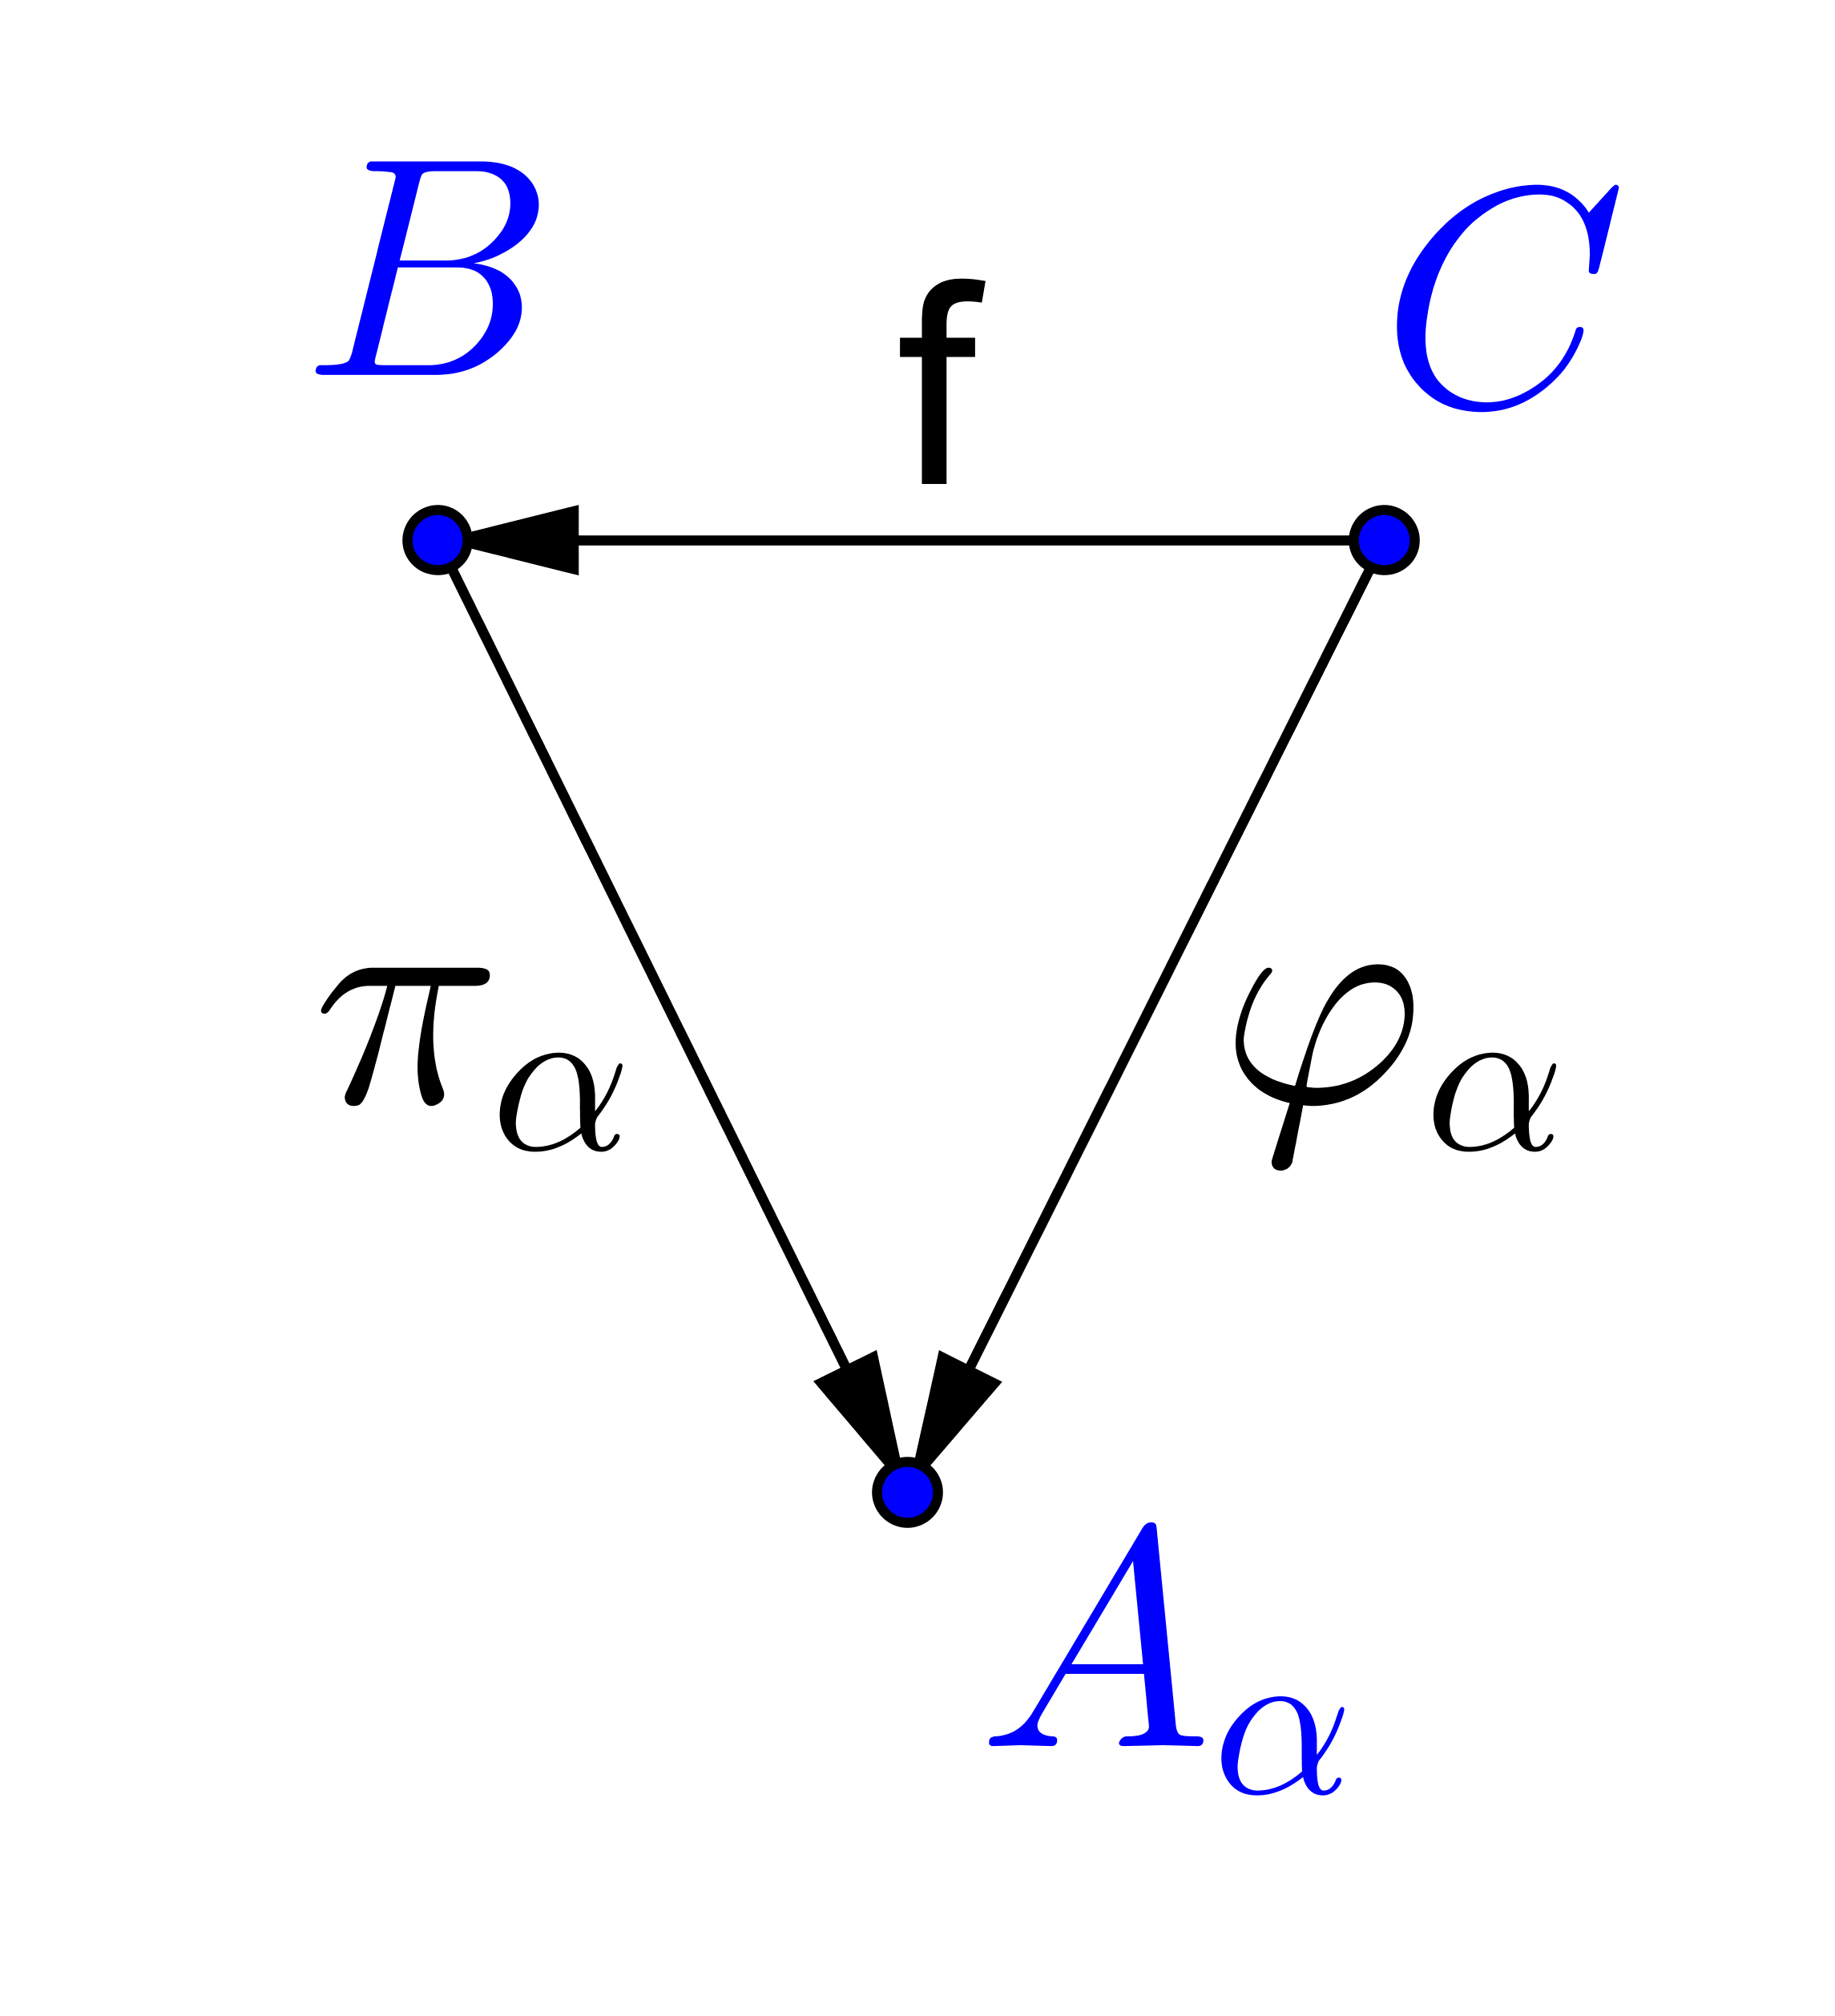
\includegraphics[width=0.3\linewidth]{lect3/FreeProduct.png}
\caption{Иллюстракция к понятию свободного произведения}
\label{fig::free_prod}
\end{figure}

На рисунке~\ref{fig::free_prod} видно, как работает это определение. Мы берем произвольное $C$ и его морфизм в произвольный $A_{\alpha}$. Тогда, имея морфизм $\pi_{\alpha}: B\rightarrow A_{\alpha}$ мы автоматически задаём единственный морфизм из $C$ в $B$. Важное замечание состоит в том, что, возможно, лектор ошибся, и перепутал свободное произведение с свободной суммой, которая будет определена в дальнейшем.

\section{Свободная сумма}
Данное понятие очень похоже по сути на понятие свободной суммы. Вы сами увидите, что конструкции практически идентичны.

\begin{definition}[Свободная сумма]
Пусть имеется $\{A_{\alpha}|\ \alpha\in\mathfrak{A}\}$~--- некоторое множество алгебраических систем. Тогда алгебраическая система $B$, порождённая системами $A_{\alpha}$, так, что гомоморфизм $g_{\alpha}: A_{\alpha} \rightarrow C$, где $C$~--- произвольная алгебраическая система, продолжается до гомоморфизма $g:\ B\rightarrow C$ называется свободной суммой и обозначается \[
\sum^*_{\alpha\in\mathfrak{A}} A_{\alpha}.
\]
\end{definition}

\begin{figure}[htbp]
\centering
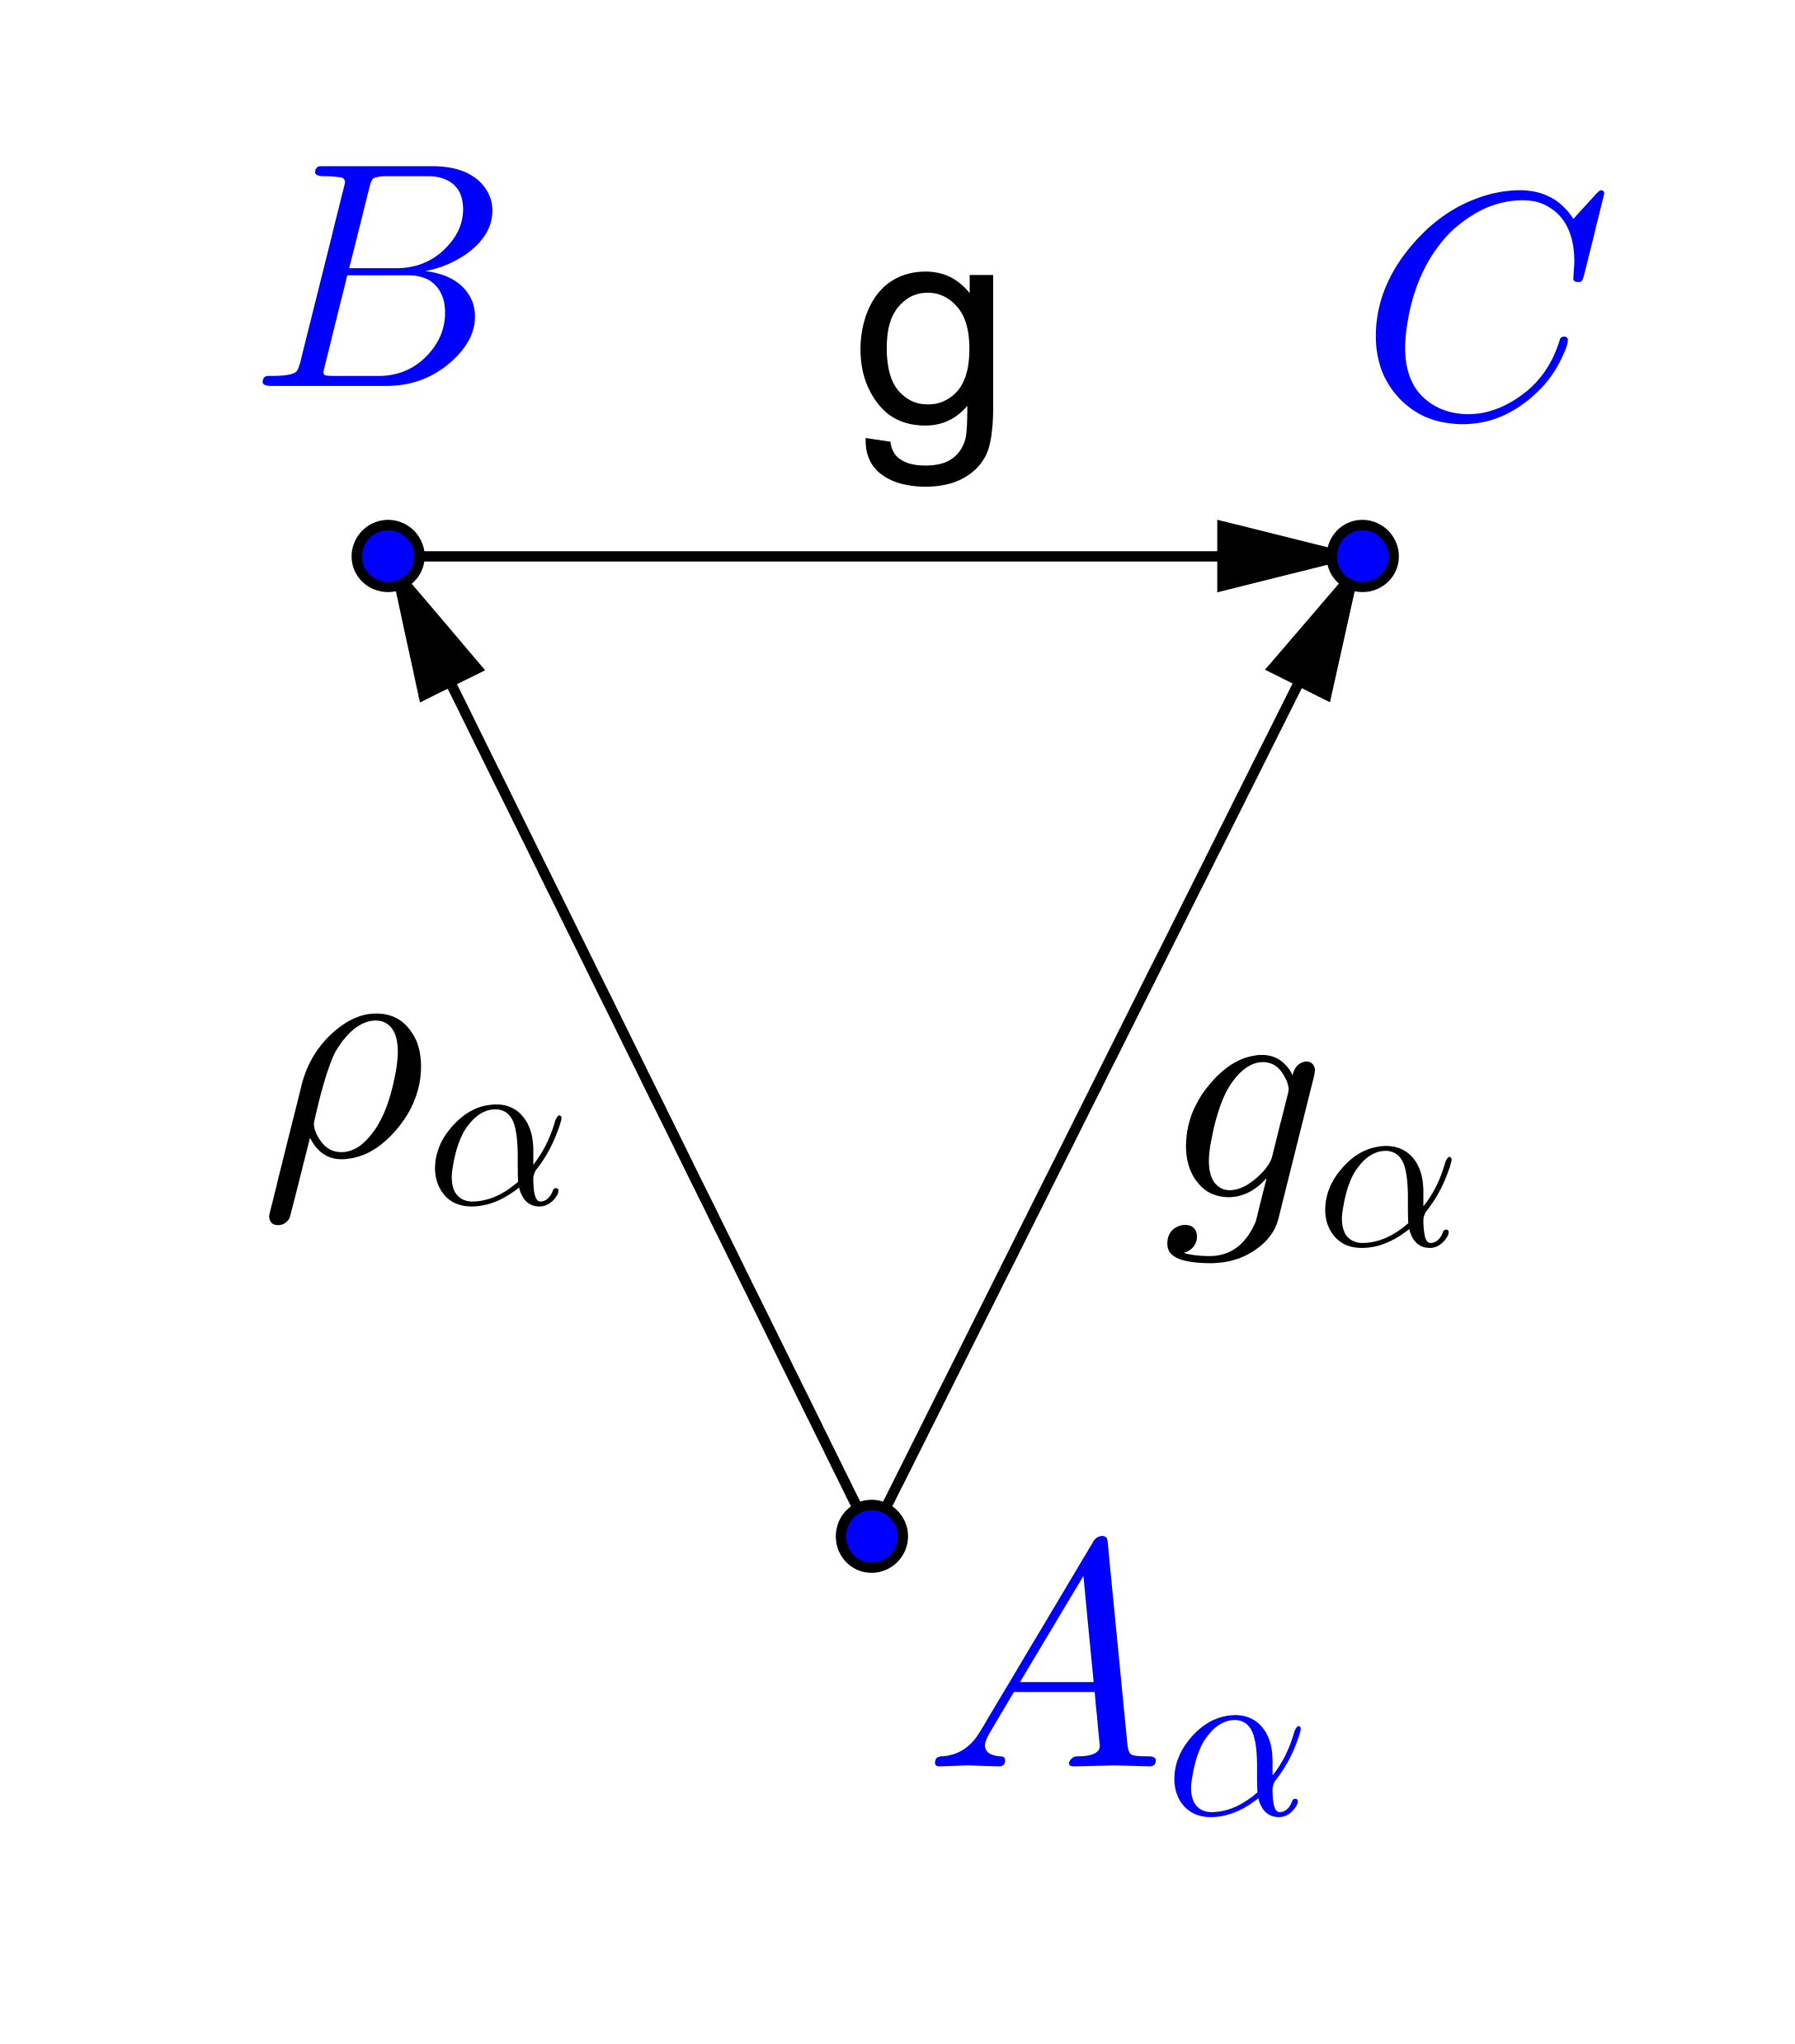
\includegraphics[width=0.3\linewidth]{lect3/FreeSum.png}
\caption{Иллюстракция к понятию свободной суммы}
\label{fig::free_sum}
\end{figure}

На рисунке~\ref{fig::free_sum} видно, как работает это определение. Его принцип очень схож с принципом свободного произведения. И на самом деле - свободная сумма двойственна свободному произведению. На всякий случай напомним понятие двойственности из теории категорий:

\begin{definition}
Двойственность в теории категорий~--— соотношение между свойствами категории $C$ и так называемыми двойственными свойствами двойственной категории $C^*$. Взяв утверждение, касающееся категории $C$, и поменяв местами образ и прообраз каждого морфизма, так же как и порядок применения морфизмов, получим двойственное утверждение, касающееся категории $C^*$. Принцип двойственности состоит в том, что истинные утверждения после такой операции переходят в истинные, а ложные в ложные.
\end{definition}

Чем же является прямая сумма в более привычных терминах теории групп? На самом деле, если множества $A_{\alpha}$ не пересекаются то это просто объединение. Если же они пересекаются, то это объединение, которое ставит в соответствие $N = \sum_{\alpha\in\mathfrak{A}} |A_{\alpha}|$ элементное множество. Например, пусть $A^*_{\alpha} = \{(a, \alpha)\| a \in A_{\alpha}\}$. Тогда $B = \bigcup A^*_{\alpha}$.

\chapter{Лекция 4}
\section{Введение в категории}
\begin{definition}
Класс~--- это объект, который не может быть элементом множества или другого класса, в остальном свойства класса и множества совпадают.
\end{definition}

\begin{definition}
Будем обозначать $\Cql(\mathfrak{U})$ пространство всех матриц над произвольным неодноэлементным множеством $\mathfrak{U}$. Заметим, что если $\mathfrak{U}$ произвольные множества, то $\Cql(\mathfrak{U})$~--- это класс.
\end{definition}

Далее введём ключевое определение данного курса.

\begin{definition}[Категория]
Будем обозначать $\Psi$ категорию. Тогда
\begin{itemize}
  \item $Ob\Psi$~--- класс
  \item $\forall (A, B) \in Ob\Psi \rightarrow Hom_{\Psi} (A, B)$~--- множество. \\ То есть любой паре элементов из $Ob\Psi$ ставится в соответствие множество отображений из $A$ в $B$.
\end{itemize}
Таким образом, категория~--- это множество объектов и операций над ними.
\end{definition}

Рассмотрим свойства категории $\Psi$.
\begin{enumerate}
  \item Пусть есть 3 элемента $A, B, C \in \Psi$ и находятся в отношениях, изображённых на рис.~\ref{fig::property_1}.
      \begin{figure}[!htbp]
        \begin{center}
            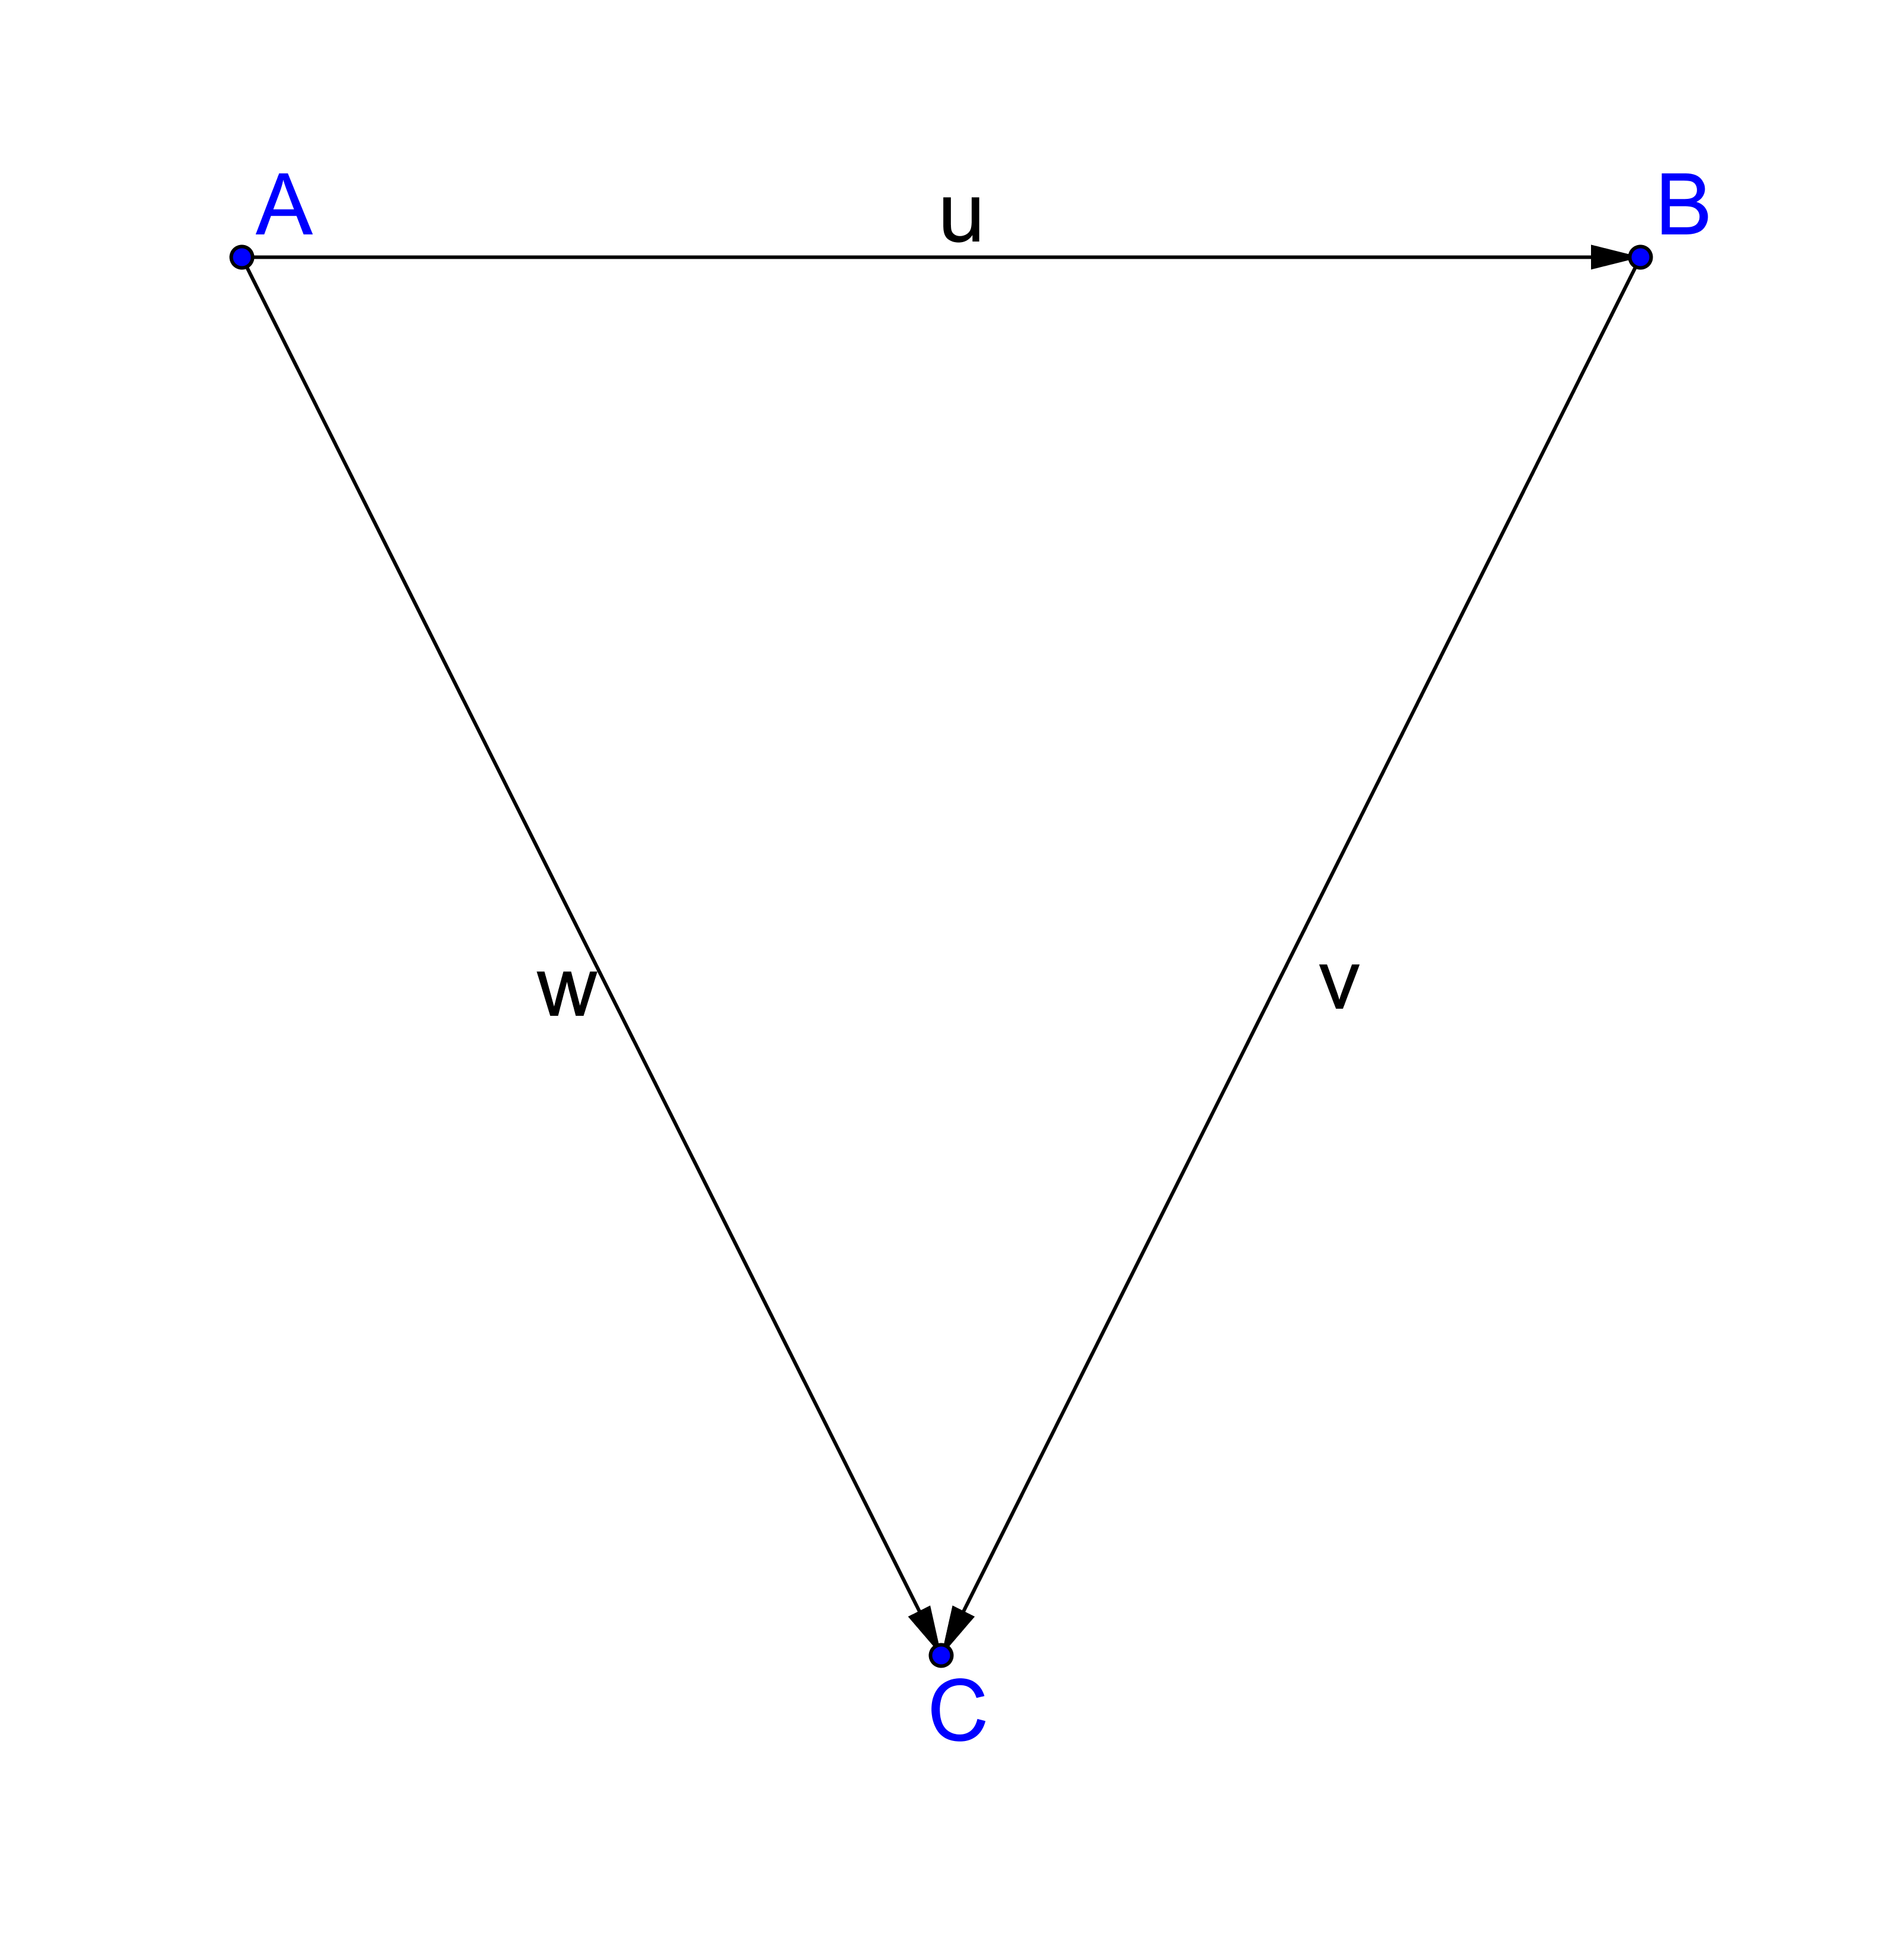
\includegraphics[width=0.3\linewidth]{lect5/Properity1pic1.png}
        \end{center}
        \caption{Отношения между объектами $A,B,C$.}
        \label{fig::property_1}
      \end{figure}

      Тогда $w = v \circ u$. Таким образом определены суперпозиции для морфизмов. Более того, $(u \circ v) \circ w = u \circ (v \circ w)$ для любых $u, v, w$ для которых такая суперпозиция имеет смысл. А также существует единственный элемент $e_A$, такой, что
      \begin{figure}[htbp]
        \begin{center}
             \begin{minipage}[h]{0,45\linewidth}
                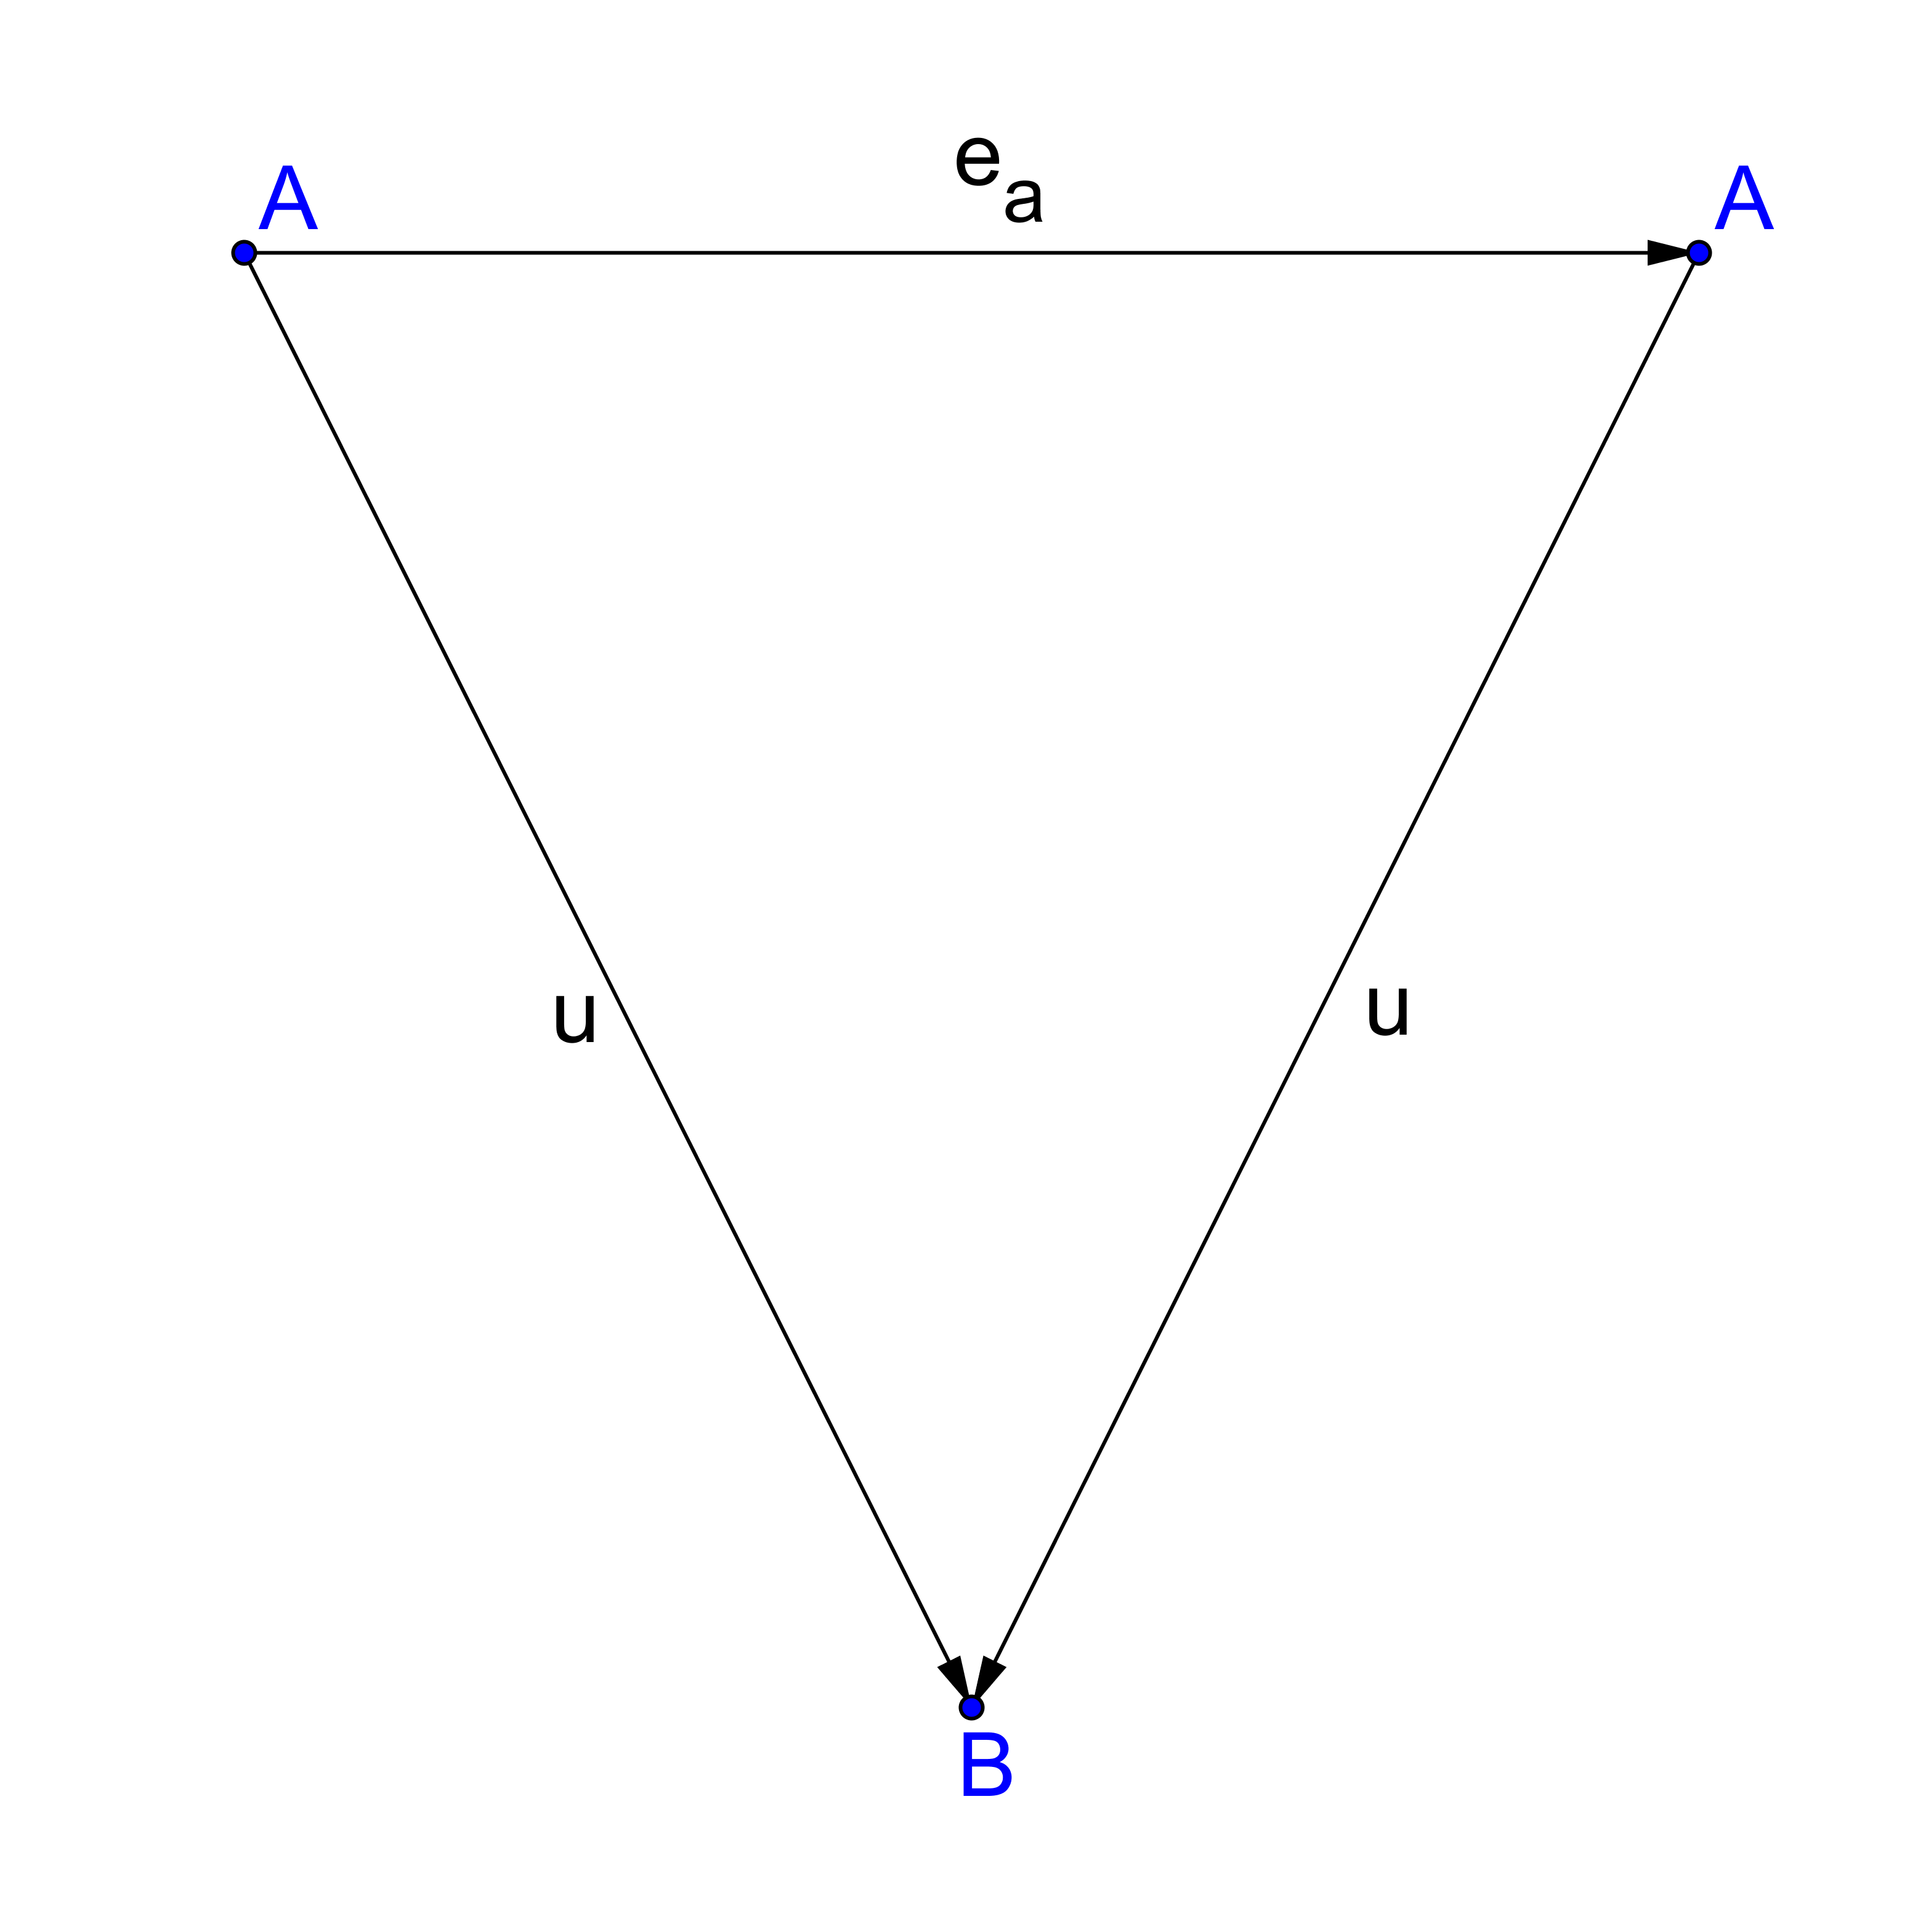
\includegraphics[width=1\linewidth]{lect5/Properity1pic2.png}
            \end{minipage}
        \hfill
            \begin{minipage}[h]{0.45\linewidth}
                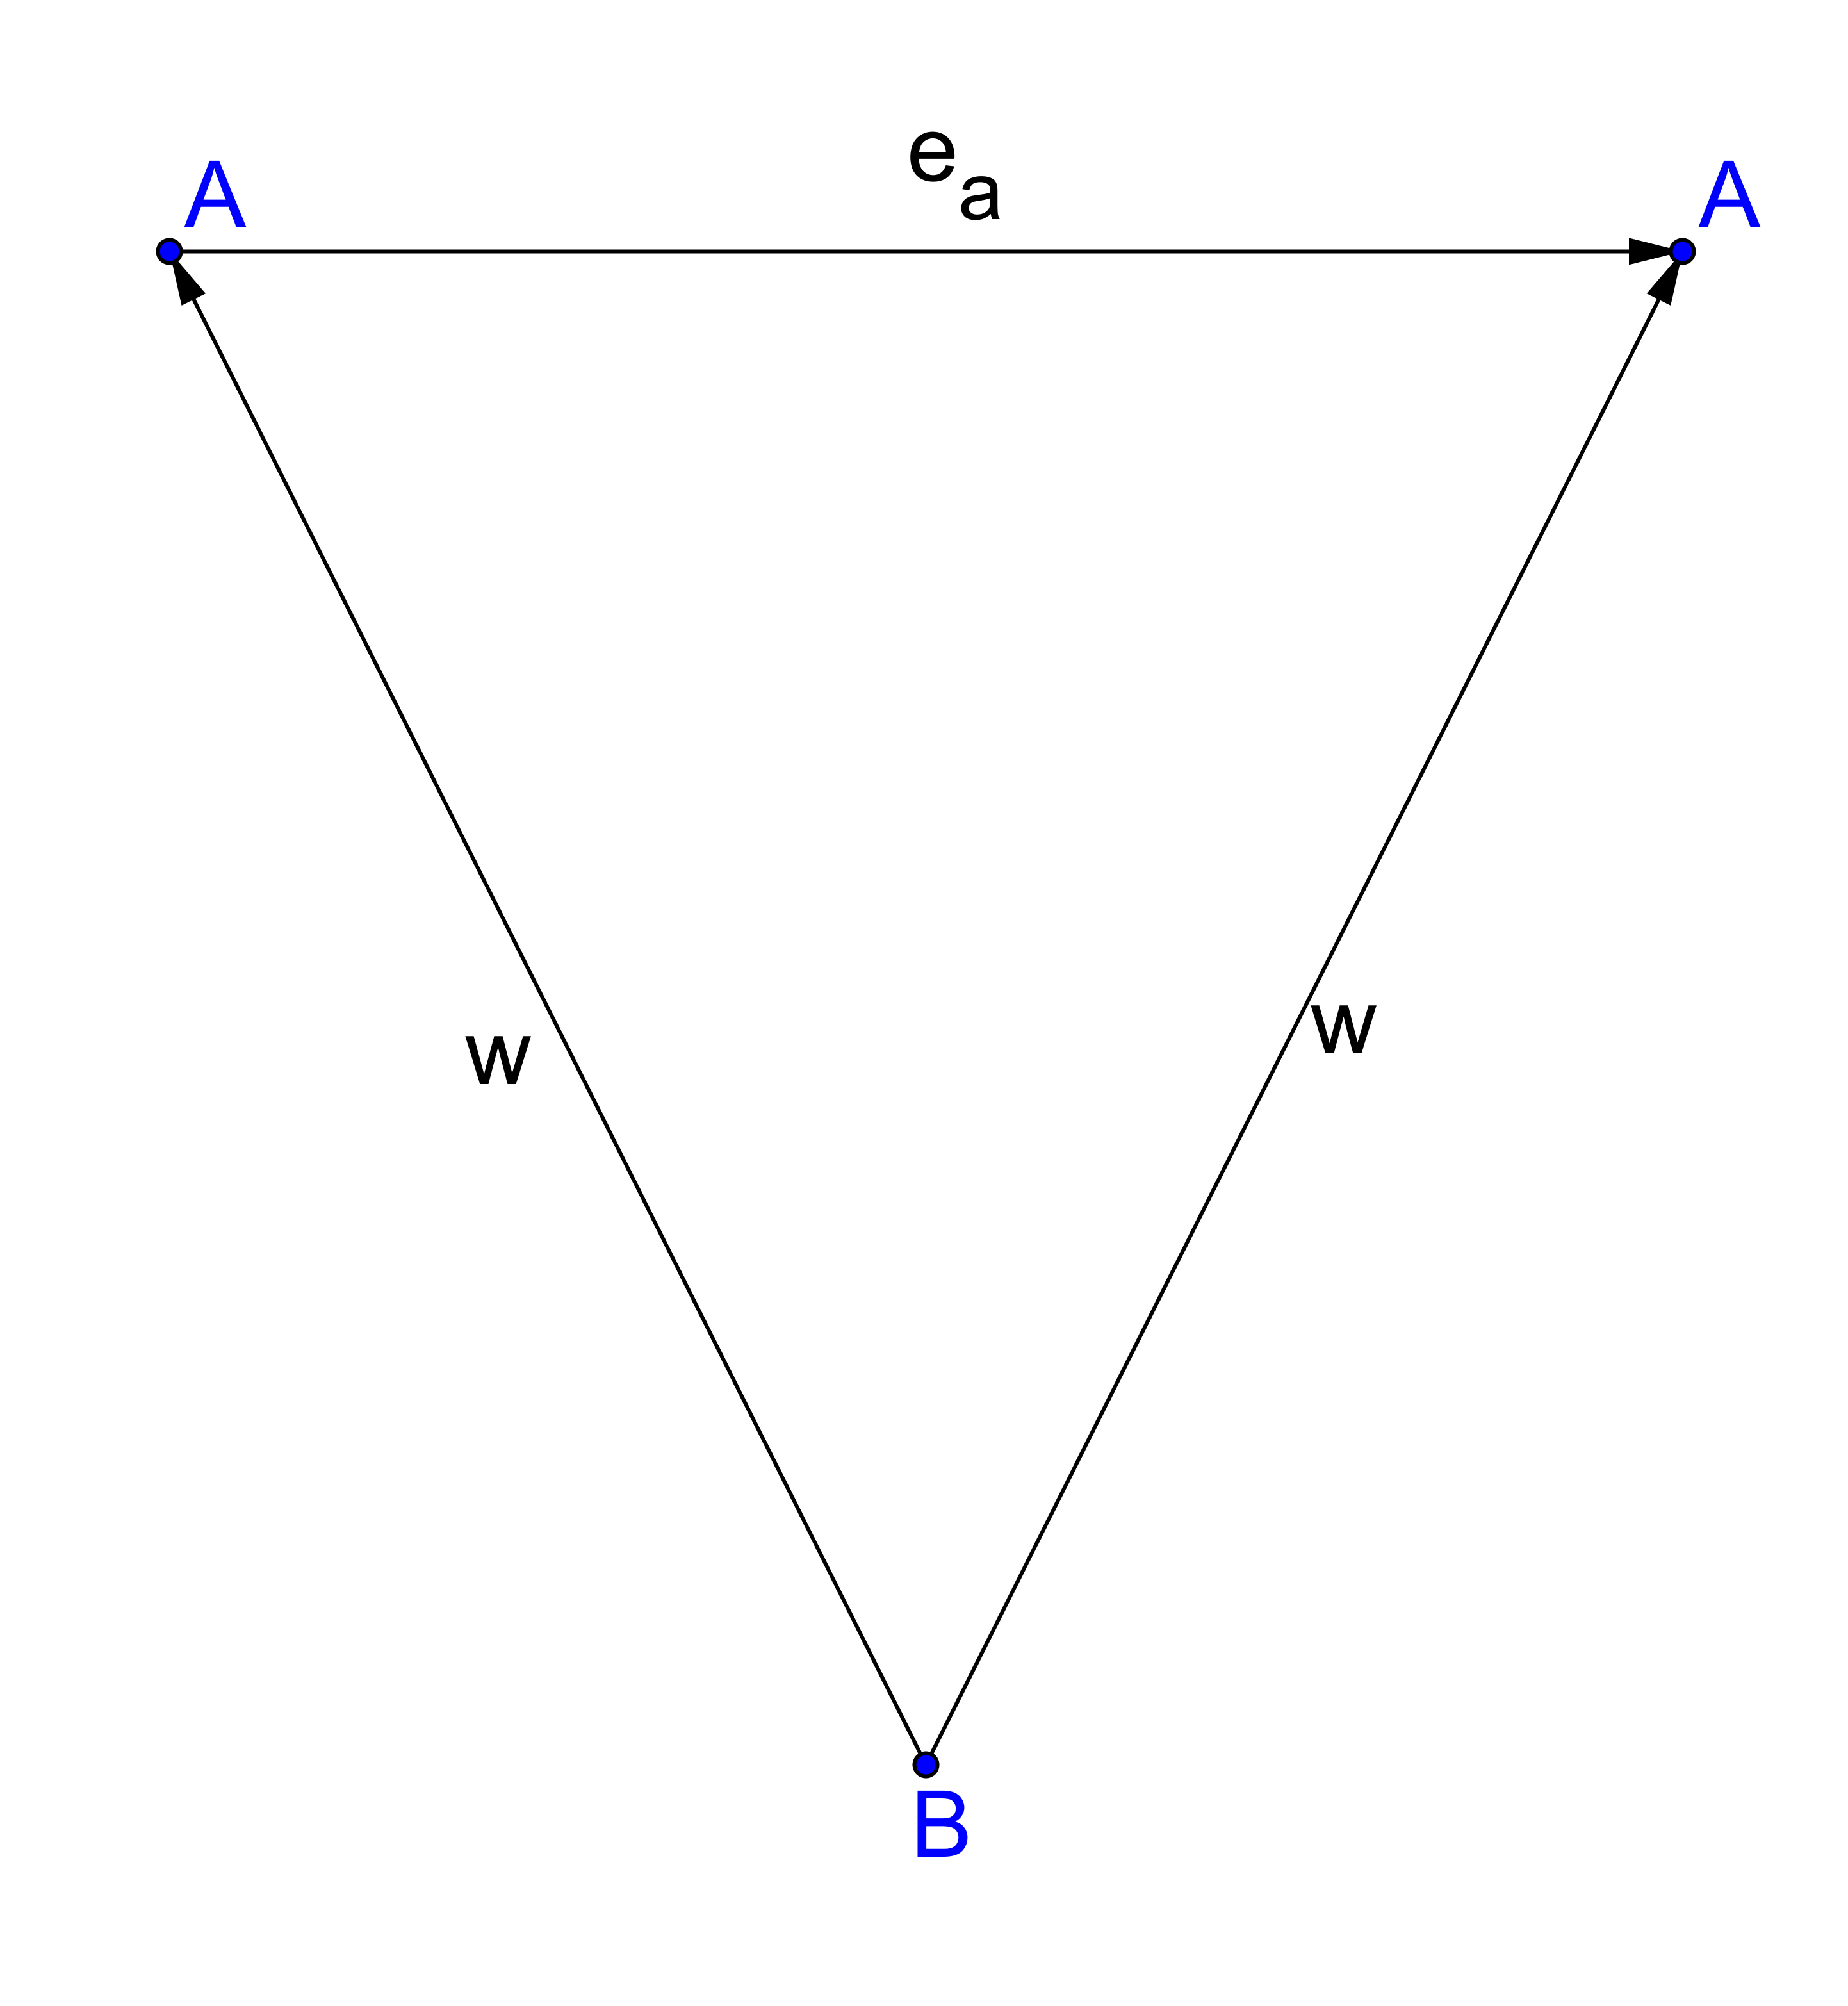
\includegraphics[width=1\linewidth]{lect5/Properity1pic3.png}
            \end{minipage}
        \end{center}
      \end{figure}
      \newpage
  \item $\Psi'$ подкатегория $\Psi$ если:
  \begin{itemize}
    \item $Ob\Psi'$~--- подкласс $Ob\Psi$
    \item $\forall\ A, B \in Ob\Psi':\ Hom_{\Psi'} \subseteq Hom_{\Psi} (A, B)$
  \end{itemize}
  Причём, если во втором условии стоит равенство, то $\Psi'$~--- полная подкатегория категории $\Psi$.
\end{enumerate}

\paragraph{Пример категории.} Объекты~--- это множества $A, B$; морфизмы~--- это отображения из $2^A$ в $2^B$. Например, отображения из $\Cql(\mathfrak{U})$ в $\Cql(\mathfrak{V})$, коммутирующие со всеми перестановками строк.


\section{Дальнейшая формализация общей задачи}
Для начала введём несколько понятий, тут будут использоваться следующие обозначения: $ob = object,\ cl=class,\ i=initial,\ f=final$.
Приступим:
\begin{itemize}
  \item $\Upsilon=\{S\}$
  \item $\mathfrak{D}_{ob}:\ \Upsilon\rightarrow\mathfrak{J}_{ob}$
  \item $K_1,\ldots,K_l;\ K_j \subseteq \Upsilon,\ j=\overline{1,l}$. Мы рассматриваем задачу классификации и $K_1,\ldots,K_l$~--- наши классы. Они являются элементами одного множества, но сами могут быть различны.
  \item $\mathfrak{D}_{cl}:\ 2^{\Upsilon}\rightarrow\mathfrak{J}_{cl}$
\end{itemize}
Наша задача:
\[
A:\ \mathfrak{J}_i \rightarrow \mathfrak{J}_f.
\]
Её решение может быть формализовано в различных вариантах:
\begin{enumerate}
  \item $\mathfrak{J}_i = \mathfrak{J}_{ob}\times\mathfrak{J}_{cl}$. В такой постановке мы игнорируем тот факт, что классов $l$ и что они однородны.
  \item $\mathfrak{J}_i = \mathfrak{J}_{ob}\times\mathfrak{J}_{cl}^l$. Этот вариант лишен проблемы первого пункта и классы наши различны.
  \item $\mathfrak{J}_i = \mathfrak{J}_{ob}^q\times\mathfrak{J}_{cl}^l$. Ещё более сложный вариант, в котором участвует количество объектов $q$. Таким образом, $S_1,\ldots,S_q$~--- объекты, $(S_1,\ldots,S_q)\in\Upsilon^q$ и окончательно $\mathfrak{D}(S_1),\ldots,\mathfrak{D}(S_q) \in \mathfrak{J}_{ob}^q$.
  \item $\mathfrak{J}_i = \Cql(\mathfrak{J}),\ \mathfrak{J}_f = \Cql(\tilde{\mathfrak{J}})$, где $\Cql$~--- пространство $q\times l$ матриц над чем-либо. Данный вариант наиболее общий, и его мы будем в дальнейшем рассматривать, считая $\mathfrak{J},\ \tilde{\mathfrak{J}}$ неодноэлементными множествами (иначе множество матриц тривиально).
\end{enumerate}

Может показаться, что пункт 4 и 3 дают одинаковую задачу, но это не так. \textcolor{red}{Саня, Я не помню контрпример. Если у тебя есть - впиши}

В новых терминах решение задачи Z формулируется таким образом. Пусть $\hat{I} \in \Cql(\mathfrak{J})$ и $\hat{\tilde{I}} \in \Cql(\tilde{\mathfrak{J}})$. Мы ищем такие отображения $A$, что они являются допустимыми и $A(\hat{I}) = \hat{\tilde{I}}$

\begin{definition}
Алгоритм называется корректным на прецедентах, если $A(\hat{I}) = \hat{\tilde{I}}$
\end{definition}
\textcolor{red}{Саня, я тут не особо хорошо записывал. Проверь. Как то странновато вышло.}

\chapter{Лекция 5}
\section{Определение инъекции и сюръекции через морфизмы}

\begin{definition}[Мономорфизм]
Отображение $u:\ A \rightarrow B$ называется мономорфизмом iff при любых $C$, $g_1$ и $g_2$, таких что $g_1:\ C \rightarrow A$, $g_2:\ C \rightarrow A$ и $g_1 \neq g_2$ выполнено $f \circ g_1 \neq f \circ g_2$ в смысле равенства элементов множества морфизмов.
\end{definition}

\chapter{Лекция 6}
\section{Переход к категориям}
Для начала введем несколько упрощающих запись обозначений:
\begin{itemize}
  \item $Hom_{\Psi}(\Cql(\frakU),\ \Cql(\frakW)) = H(\frakU,\ \frakW)$
  \item $\bigcup_{p=0}^{\infty}Hom_{\Psi}(\Cql^p(\frakU),\ \Cql(\frakW)) = \calH(\frakU,\ \frakW)$
\end{itemize}
\textcolor{red}{Саня, Я не нашёл нужную букву под фигурное W. Пока что там стоит mathfrak{W}}
\begin{definition}
Категория $\Psi$ называется полной категорией, если при любых неодноэлементных $\frakU$ и $\frakV$ выполнено
\[
\calH(\frakU, \frakV)(\Cql(\frakU)) = \Cql(\frakV).
\]
\end{definition}

Определим также понятие регулярной задачи. Пусть у нас есть множество $\mathfrak{Z}=\{Z\}$ - множество задач Z. Регулярность можно определять несколькими способами, например:
\begin{definition}[Регулярность по Журавлеву]
Задача регулярна, если разрешима для любой $\htI$.
\end{definition}
\begin{definition}
Задача называется регулярной, если существует окрестность $O(Z)\subseteq \mathfrak{Z},\ Z\in O(Z)$ такая, $\forall Z_i\in O(Z) \rightarrow Z_i$ - разрешима.
\end{definition}
Мы будем пользоваться вторым определением.
Таким образом каждой задаче $Z$ задан в соответствие набор $((\hI,\ \htI), I_{str}^u)$, $O(Z) = \{Z'| Z' \leftrightarrow ((\hI,\ \htI'), I_{str}^u)\}$.
И окончательно $I_{str} \leftrightarrow \Psi$.
\textcolor{red}{Саня, итак, получилось уберкоротко и нихрена не понятно (частично понятно, но последняя строчка вообще хрен знает откуда вылезла) Плюс я картинку не рисовал (квадрат со стрелочками). Надо с обозначениями для них разобраться.}

\chapter{Лекция 7}
\section{Понятие базы и формализация требований к морфизмам}
Нам потребуется понятие базы для последующих исследований. Введем его схожим с линейными пространствами способом:
\begin{definition}
Множество $X\subseteq \Cql(\frakU)$ называется базой в $\Psi$, если $\calH(\frakU,\frakU)(X)\ =\ \{\hfrakU| \hfrakU \in \Cql(\frakU),\ \exists p\ \exists U\ \exists_{X^p} (\hfrakU^1,\ldots,\hfrakU^p): \hfrakU = u(\hfrakU^1,\ldots,\hfrakU^p)\}$. \\
Данная развернутая запись является обобщением простой идеи:  $\calH(\frakU,\frakU)(X) = \Cql(\frakU)$. \\
Или ещё проще - из множества $X$ с помощью всех морфизмов из $\Psi $можно получить любую матрицу из $\Cql(\frakU)$.
\end{definition}
Однако, этого определения нам недостаточно, так как в нашей задаче мы смотрим морфизмы из одного множества в другое. Поэтому нам нужно множество $X$ в первом множестве, являющееся базой во втором. Это приводит нас к следующему определению.
\begin{definition}
Множество $X\subseteq \Cql(\frakU)$ называется базой в $\Cql(\frakU)$ для $\Cql(\frakW)$, если $\calH(\frakU,\frakW)(X) = \Cql(\frakW)$.
\end{definition}
Также, для предстоящей нам теоремы нам потребуется понятие полной категории.
\begin{definition}
$\Psi$~--- полная категория, если при всех $\frakU$ и  $\frakW$: $\calH(\frakU,\frakW)(\Cql(\frakU)) = \Cql(\frakW)$.\\
Иначе, если $\Cql(\frakU)$ база в $\Cql(\frakU)$ для $\Cql(\frakW)$.
\end{definition}

Всё это приводит нас к следующей теореме.
\begin{theorem}
Пусть $\Psi$ - полная допустимая категория, $\frakU,\ \frakW$ - множества. Тогда $(X$ - база$)\Leftrightarrow(X$ - база в $\Cql(\frakU)$ для $\Cql(\frakW))$.
\end{theorem}
\begin{proof}
\textbf{I) Необходимость.} Пусть $X$ - база. Возьмём $\hat{V} \in \Cql(\frakW)$ и покажем, что мы можем получить его из элементов $X$ с помощью морфизмов из $\Psi$. \\
Так как $\Psi$~--- полна $\rightarrow\ \exists p \in \mathds{N}\ \exists u \in Hom_{\Psi}(\Cql^p(\frakU), \Cql(\frakW))\ \exists \hu^1,\ldots,\hu^p \in \Cql^p(\frakU):\ \hat{V} = u(\hu^1,\ldots,\hu^p)$. \\
И $\forall k\in\{1,\ldots,p\}\ \exists u_k \in \calH(\frakU, \frakU)\ \exists \hu'^1_k,\ldots,\hu'^{n_k}_k \in X^{n_k}:\ \hu^k = u_k(\hu'^1_k,\ldots,\hu'^{n_k}_k)$.\\
Подставим в выражение $\hat{V} = u(\hu^1,\ldots,\hu^p)$ выражения для $\hu^i$. Таким образом, получим:\\
$\hat{V} = u(u_1(\hu'^1_1,\ldots,\hu'^{n_1}_1,\ldots,u_p(\hu'^1_p,\ldots,\hu'^{n_p}_p))) = u\circ(u_1\times\ldots\times u_p)(\hu'^1_1,\ldots,\hu'^{n_p}_p)$. \\
Ввиду допустимости категории $\Psi$, морфизм $u\circ(u_1\times\ldots\times u_p) \in \Psi$ и мы получили с помощью морфизмов $\Psi$ любой элемент из $\Cql(\frakW)$. \\

\textbf{I) Достаточность.} Пусть $(X$ - база$)\Leftrightarrow(X$ - база в $\Cql(\frakU)$ для $\Cql(\frakW))$. Тут будем действовать практически аналогично пункту с необходимостью. \\
Возьмем $\hat{U} \in \Cql(\frakU)$. Поскольку $\Psi$~--- полна, то $\hat{U} = u(\hv^1,\ldots,\hv^p)$ и $\hv^k = v_k(\hv'^1_k,\ldots,\hv'^{n_k}_k)$, причём все $\hv'^i_j \in X$.\\
Таким образом    $\hat{U} = u(v_k(\hv'^1_1,\ldots,\hv'^{n_1}_1),\ldots,v_k(\hv'^1_p,\ldots,\hv'^{n_p}_p)) = v\circ(v_1\times\ldots\times v_p)(\hv'^1_1,\ldots,\hv'^{n_p}_p)$.\\
Ввиду допустимости категории $\Psi$, морфизм $v\circ(v_1\times\ldots\times v_p) \in \Psi$ и мы получили с помощью морфизмов $\Psi$ любой элемент из $\Cql(\frakU)$.
\end{proof}

\chapter{Лекция 8}

\begin{definition}
Операция $\frakm'$ корректна, если $\frakm'(\Cql(\calR)) = \Cql(\tilde{\frakI})$.
\end{definition}

\begin{definition}
Справедливы следующие отношения:
\[
f\text{-полно} \Leftrightarrow f\text{-}\Gamma\text{-полно} \Leftrightarrow X\text{-база} \Rightarrow f(X) = \Cql(\calR).
\]
\end{definition}

Отображение $\frakm$ представимо в следующем виде:
\[
\frakm = \frakm' \circ f \circ \frakm^0.
\]

Рассмотрим множество $S = \{ (1, 1), \ldots, (q,l) \}$ и симметрическую группу подстановок $\sigma_0$, действующую на множестве $S$. Обозначим $s \in \sigma_0$ отображение $s: \Cql^p(\frakU) \rightarrow \Cql^p(\frakU)$.

\begin{definition}
$s(\hat{u}) = s(\| \hat{u}_{ij} \|_{q\times l}) = \|\hat{u}_{s(i, j)} \|_{ql}$
\end{definition}

\begin{definition}
$s(\hat{u}^1, \ldots, \hat{u}^p) = (s(\hat{u}^1), \ldots, s(\hat{u}^p))$
\end{definition}

\begin{definition}
Пусть $u: \Cql(\frakU) \rightarrow \Cql(\frakW)$ и $s \in \sigma_0$. Тогда $u$ коммутирует с $s$, если $u \circ s = s \circ u$.
\end{definition}

\begin{definition}
Категория $\Delta$~--- подкатегория $\Psi_{ql}$, такая что при всех множествах $\frakU$ и $\frakW$, арностях $p_1$ и $p_2$ множество морфизмов
\[
Hom_{\Delta}(\Cql^{p_1}(\frakU), \Cql^{p_2}(\frakW)) = \{ u: \Cql() \rightarrow \Cql(), \; \forall s \in \delta \subseteq \sigma_0: \; u \circ s = s \circ u \}.
\]
\end{definition}

Проверка требований к категории:
\begin{enumerate}
\item Тождественное отображение коммутирует с любым отображением.
\item Коммутация суперпозиций: $(u \circ v) \circ s = u \circ (v \circ s) = u \circ (s \circ v) = s \circ (u \circ v)$.
\end{enumerate}
Допустимость категории следует из определения.

\begin{St}
$\forall us_1 = s_1u$ {\rm и} $us_2 = s_2u \Rightarrow u(s_1s_2) = (s_1s_2)u$
\end{St}

Если $\delta \subseteq \sigma_0$ и $\sigma_{\delta}$~--- подгруппа, для которой $\delta$ образующая, тогда $\Delta = \Delta_{\delta}$.

Если $\delta_1 \subseteq \delta_2 \Rightarrow \Delta_2$~--- подкатегория $\Delta_1$: добавление ограничений на $u$ из определения~$\Delta$. Следовательно, $\sigma_0$ соответствует минимальной категории, так как накладывается наибольшее количество ограничений.

Примеры морфизмов категории $\Sigma_0$:
\begin{enumerate}
\item Сложение действительных матриц.
\item Поэлементное умножение матриц.
\item Нормировка матрицы. В отличии от двух предыдущих примеров зависит целиком от всей матрицы, а не от пары элементов.
\end{enumerate}
\chapter{Лекция 9}
\begin{St}
Категория $\Sigma_0$ полна.
\end{St}
\begin{proof}
Нужно доказать, что $\forall \frakU, \frakV$: $\calH(\frakU, \frakV)(\Cql(\frakU)) = \Cql(\frakV)$.
\end{proof}

Матрица с попарно различными элементами~--- одноэлементная база.


\chapter{Лекция 10}
\begin{St}
Пусть $\sigma \subseteq \sigma_0$, $\Sigma$ категория, соответствующая $\sigma$, $\frakU$~--- некоторое множество и $X \subseteq \Cql(\frakU)$. Тогда
\[
X\text{~--- база категории} \; \Sigma \Leftrightarrow \forall s \in \sigma \setminus \{e\} \ \exists \hat{u} \in X: s(\hat{u}) \neq \hat{u}.
\]
\end{St}
\begin{proof}
Идея доказательства: если есть нетождественная подстановка переводящая все матрицы в себя, то нельзя получить всё пространство.

\textbf{Необходимость.} Пусть $\exists s \in \sigma \setminus \{e\}: \forall \hat{u} \in X$ выполнено $s(\hat{u}) = \hat{u}$. Рассмотрим такую матрицу $\hat{v} \in \Cql(\frakV)$, что $s(\hat{v}) \neq \hat{v}$. Матрица $\hat{v}$ найдётся, так как $s$ нетождественна, следовательно существуют элементы, которые перемещаются по орбите, длина которой больше 1; составим $\hat{v}$ из различных элементов множества $\frakV$, стоящих на позициях, соответствующих этой орбите.

Пусть $u$~--- морфизм $\Sigma$: $\exists \hat{u}^1, \ldots \hat{u}^p \in X^p$ такие что
\[
u(\hat{u}^1, \ldots, \hat{u}^p) = \hat{v}.
\]
Подействуем на последнее равенство перестановкой $s$:
\begin{equation*}
\begin{split}
& s \circ u(\hat{u}^1, \ldots, \hat{u}^p) = s(\hat{v}) \neq \hat{v}\\
& u \circ s(\hat{u}^1, \ldots, \hat{u}^p) = u(s(\hat{u}^1), \ldots, s(\hat{u}^p)) = u(\hat{u}^1, \ldots, \hat{u}^p) = \hat{v}
\end{split}
\end{equation*}
Получили противоречие с принадлежностью $u$ к морфизмам категории $\Sigma$.

\textbf{Достаточность.} Пусть $\sigma \setminus \{e\} = (s_1, \ldots, s_p)$~--- подстановки из группы $\sigma$. Пусть вектор матриц $\bar{\hat{u}}^0 = (\hat{u}^1, \ldots, \hat{u}^p)$ такой, что выполнено условие
\[
s_k(\hat{u}^k) \neq \hat{u}^k. \eqno(*)
\]
Отсюда выполнено $\forall k s_k(\bar{\hat{u}}) \neq \bar{\hat{u}}$: если есть несовпадение в элементе вектора, то вектора не совпадают.

Пусть $\hat{v} \in \Cql(\frakV)$. Построим $u: \Cql^p(\frakV) \rightarrow \Cql(\frakV)$ следующим образом:
\[
u_{\hat{v}}(\hat{u}^{'1}, \ldots, \hat{u}^{'p}) = u_{\hat{v}}(\bar{\hat{u}}') =
\begin{cases}
s(\hat{v}),\; \text{при} \; \bar{\hat{u}}' = s(\bar{\hat{u}}^0) \; \forall s \in \sigma\\
\hat{V}^0 = \| v^0 \|, \; \text{при всех} \; s \in \sigma: \ \bar{\hat{u}}' \neq s(\bar{\hat{u}}^0),
\end{cases}
\]
где $\bar{\hat{u}}'$~--- произвольный вектор матриц из $\Cql(\frakV)$, $\hat{V}^0 = \| v^0_{ij} \| = \| v^0 \|$ и $v^0 \in \Cql(\frakV)$, поэтому $\hat{V}^0$ коммутирует со всеми перестановками. В первом условии стоит $s(\cdot)$, потому что равенство должно достигаться не только в точке, но и на всех перестановках.

Условие (*) необходимо для корректного определения функции для первого случая, иначе можно было бы в одной точке определить функцию по-разному.

Проверим, что $u_{\hat{v}}$ коммутирует с $s$\footnote{Сева, зачем нам нужно это? Как связать с категорией?}: $s \circ u_{\hat{v}} = u_{\hat{v}} \circ s$.
\begin{enumerate}
\item Если $\bar{\hat{u}}' = s_0(\bar{\hat{u}}^0)$, тогда $s \circ u_{\hat{v}}(s_0(\bar{\hat{u}}^0)) = s \circ s_0(\hat{v})$ и $u_{\hat{v}} \circ s(s_0(\hat{u}^0)) = u_{\hat{v}}(s \circ s_0(\bar{\hat{u}}^0)) = s \circ s_0(\hat{v})$.
\item Если $\bar{\hat{u}}' \neq s(\bar{\hat{u}}^0) \; \forall s$, то $s(s_0(\hat{v}^0)) = \hat{v}^0 = ss_0(v^0)$.
\end{enumerate}
\end{proof}
Пример.
\end{document} 